\chapter{Integration strategy}
This section describes decisions and criteria chosen for the ITP of the system of “PowerEnJoy”.

\section{Entry criteria}
Before starting the Integration Testing phase, it is necessary to have successfully completed the Unit Testing of all the modules of the software.
So from now on we assume that all the single modules of the system of PowerEnJoy work correctly.
In addition to that we need some prerequisites to be satisfied:
\begin{itemize}
\item The software of PowerEnJoy must be code-completed.
\item The system must satisfy all the requirements of the RASD and all the decisions taken in the DD.
\item The Database should be ready and its tables are populated with initial data.
\end{itemize}

\section{Elements to be integrated}
The following image represents the Component View of the system of PowerEnJoy, as it has been designed in the DD.
We bring it here again because it clearly shows all the components of Power EnJoy that are going to be tested for integration and all the dependences existing between them.
These dependencies are particularly important because they give us a guideline to follow identifying the Integration Testing Strategy.

\begin{minipage}{\textwidth}
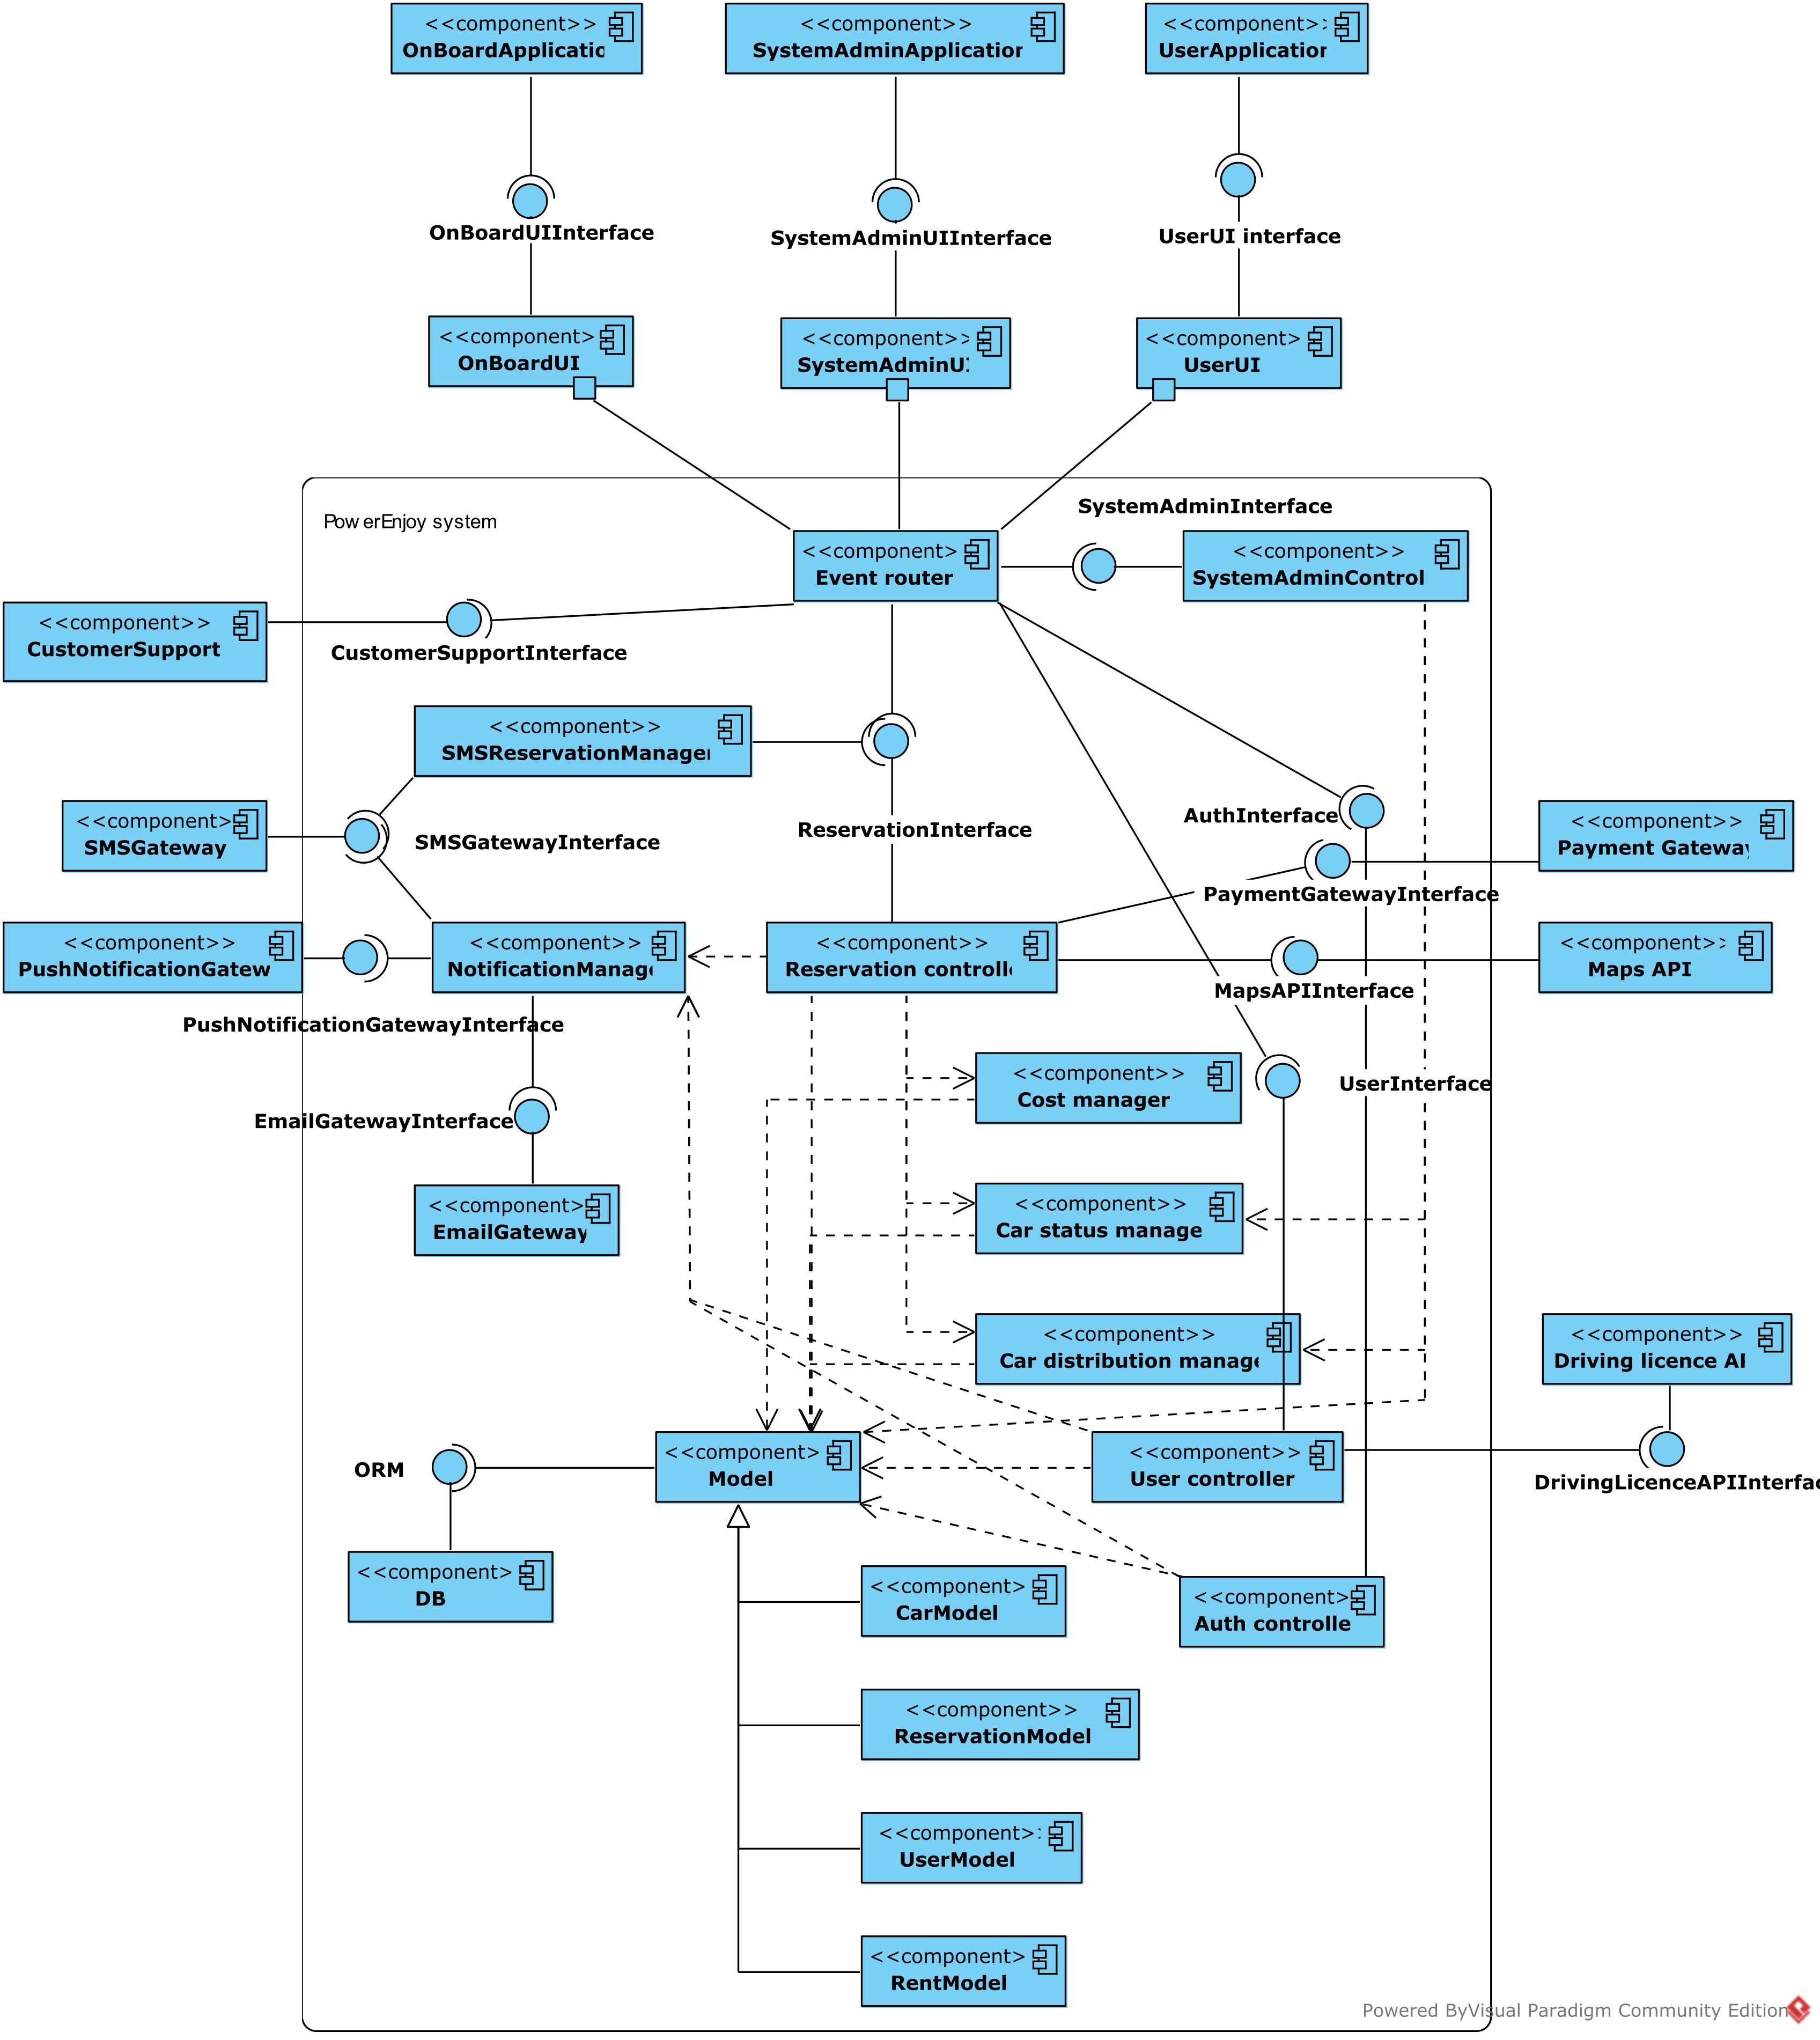
\includegraphics[width=\textwidth, keepaspectratio]{../images/diagram/component_view.png}
\captionof{figure}{Component diagram}
\end{minipage}

\section{Integration Testing Strategy}
We decide to adopt a Bottom Up approach in order to test the integration of modules of the system of PowerEnJoy.
Bottom-up testing is a type of integration testing that integrates code units and tests them together, before testing the entire system.
In this approach testing is conducted from sub module to main module, if the main module is not developed a temporary program called ‘driver’ is used to simulate the main module.
For example if we look at the following figure, first of all we test module 4, 5, 6 and 7 individually using drivers.
Then we test module 2 such that it calls 4 and 5 separately.
If an error occurs we know that there is a problem in one of the modules, or in the interface between them.
Then we test module 1 such that it calls module 3 and again if an error occurs we know that the problem is in module 3 or in the interface between module 1 and module 3.

//IMMAGINE BOTTOM-UP

\section{Sequence of Component/Function Integration}
The bottom up strategy provides a simple workflow to test modules and makes easier the formulation and the observation of tests.
Since the application has been developed, it is possible to run tests returning on the tree of modules, without creating fake contexts of execution to support the tests.

This document wants to offer a testing plan based on a particular sequence to follow, explained in detail in the next paragraph.

\subsection{Software Integration Sequence}
The sequence of integration tests depends on the strategy used to verify the correctness of tests.
In this case, the bottom up strategy has the advantage of providing simple creation of conditions of the test.

\begin{minipage}{\textwidth}
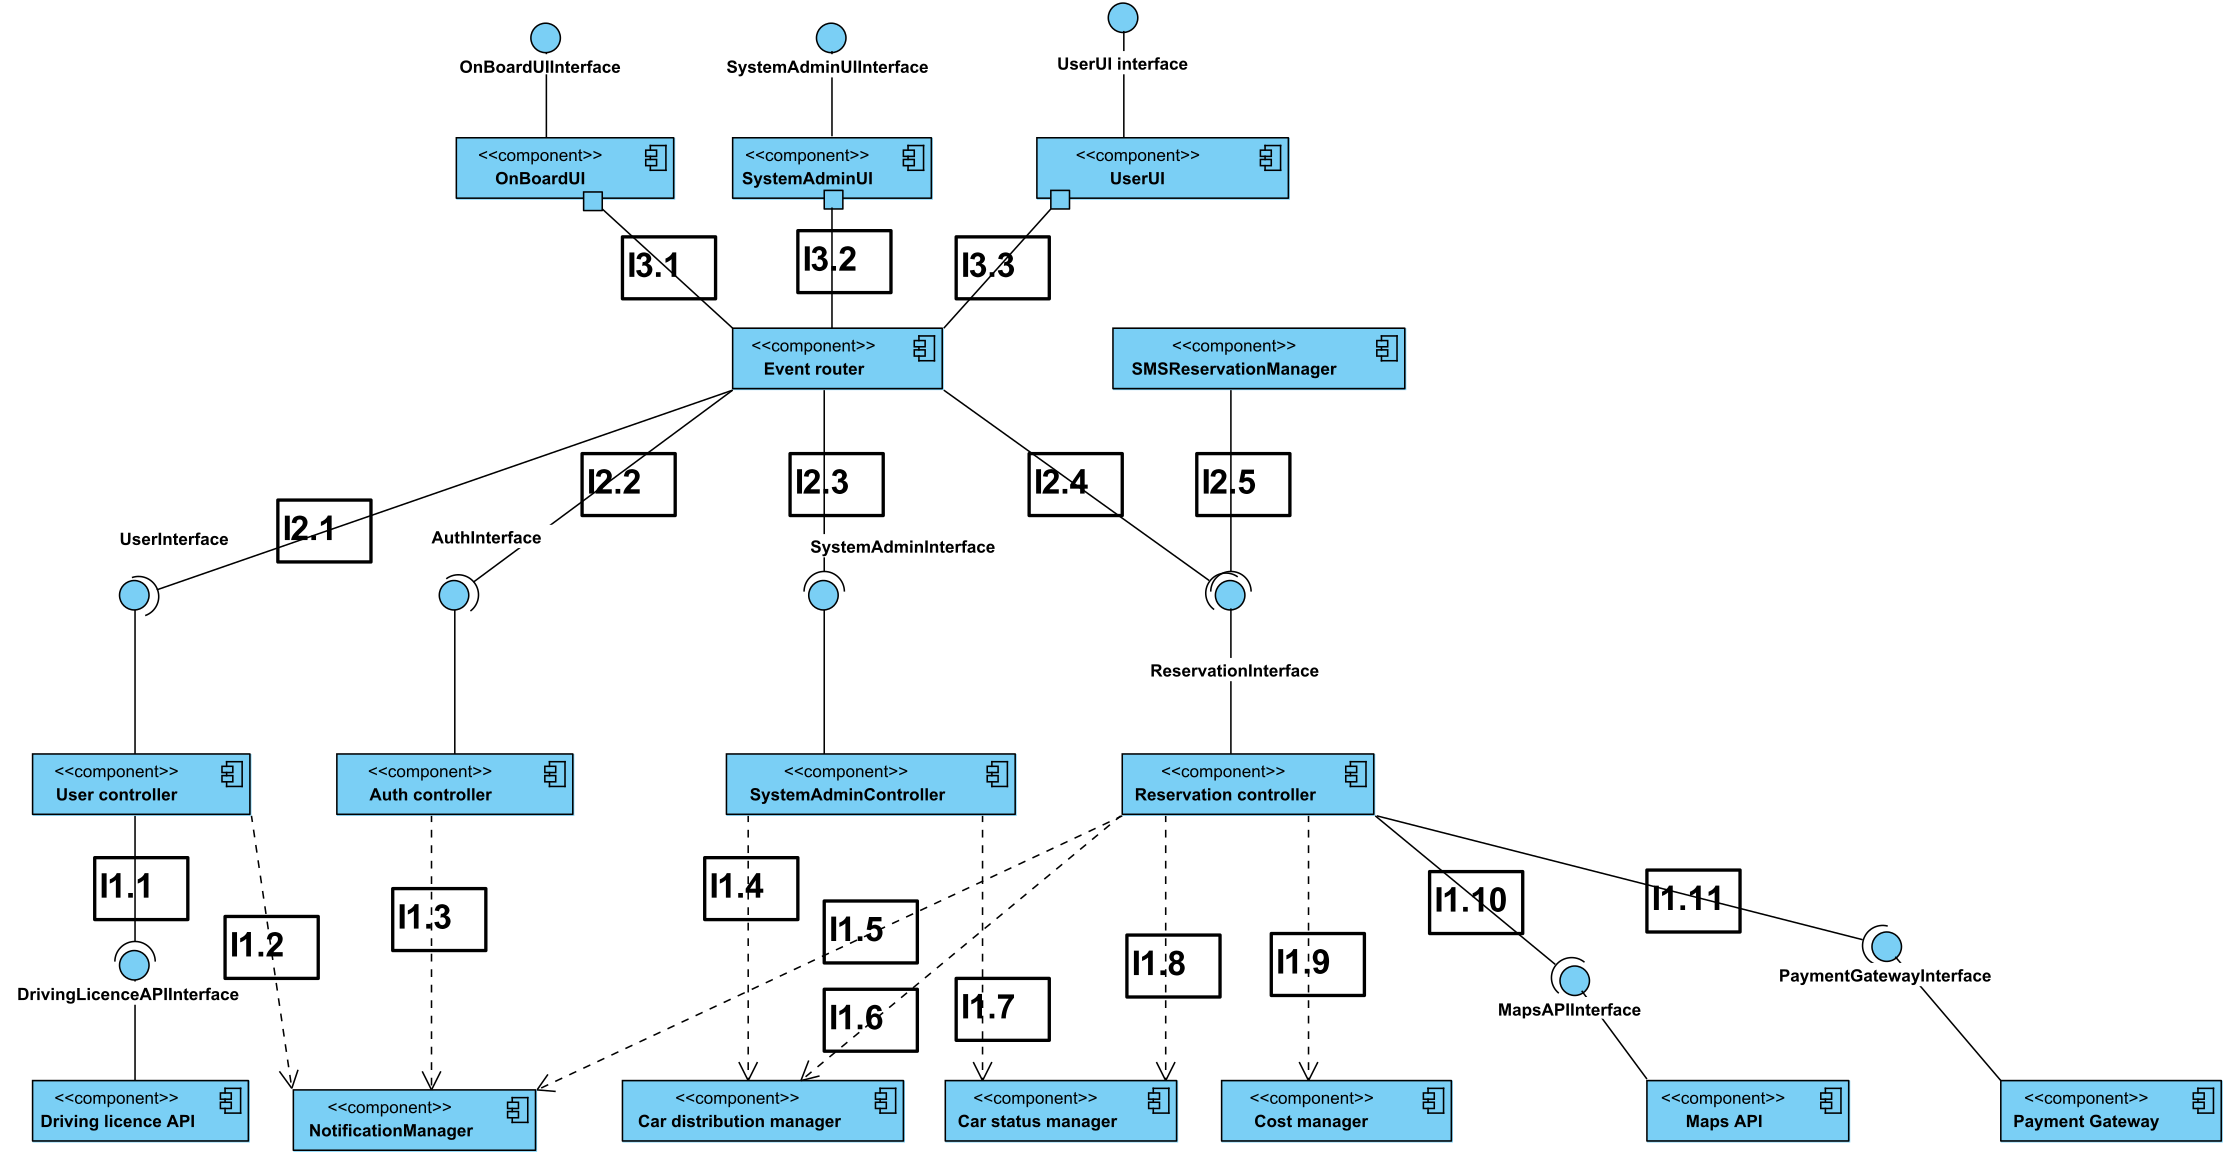
\includegraphics[width=\textwidth, keepaspectratio]{../images/diagram/integration_sequence.png}
\captionof{figure}{Integraton tests sequence}
\end{minipage}

The order to follow is based on the type of component we are going to test:
\begin{itemize}
\item \textbf{Manager components} are the most important to be tested, because they represent the logic of the application; managers must be tested with specific inputs and various test environments to guarantee as much as possible the coverage of all the cases of the domain. It’s suggested to start tests from easier functions/processes to more complex ones: in this way the next-level test can be run with no prerequisites on the atomic actions required.
\item \textbf{Gateway components} are tested when the model and the controllers work as expected. Calls to external services could require an answer to the previous request: the services we call have a particular service for tests and return us always a positive answer. Processes at this point involve an important number of components: as before, start from easier to more complex ones.
\item \textbf{UI components} are the last type of component to be tested because if each test has been positively passed before, we expect to have no surprise in the presentation of processed data. The order to follow is the same of the workflow present in the BCE.

\end{itemize}




